\documentclass[xcolor={dvipsnames}]{beamer}

\mode<presentation> {
    \usepackage[utf8]{inputenc}
    \usepackage[T1]{fontenc}
    \usepackage[english]{babel}
    \usepackage{csquotes}

    \bibliographystyle{plain}

    \usetheme{Madrid}
    \usecolortheme{ipbutfpr}

    \setbeamertemplate{caption}[numbered]
    \setbeamertemplate{bibliography item}{\insertbiblabel}
    \setbeamertemplate{frametitle continuation}{\gdef\beamer@frametitle{}}

    % \setbeamertemplate{footline}{
    %     \leavevmode%
    %     \hbox{%
    %         \begin{beamercolorbox}[wd=.4\paperwidth,ht=2.25ex,dp=1ex,center]{author in head/foot}%
    %             \usebeamerfont{author in head/foot}\insertshortauthor
    %         \end{beamercolorbox}%
    %         \begin{beamercolorbox}[wd=.6\paperwidth,ht=2.25ex,dp=1ex,center]{title in head/foot}%
    %             \usebeamerfont{title in head/foot}\insertshorttitle\hspace*{6em}
    %             \insertframenumber{} / \inserttotalframenumber\hspace*{1ex}
    %         \end{beamercolorbox}
    %     }%
    %     \vskip0pt%
    % }

    \setbeamertemplate{navigation symbols}{}
}

\usepackage[language=brazil, style=numeric, sorting=none]{biblatex}
\addbibresource{main.bib}
\makeatletter

\makeatother

\title[Placement Dashboard]{PLACEMENT DASHBOARD}

\author[Bhumika, Vaishnavi]{Bhumika Saxena and Vaishnavi Janardhan}

\institute{TalentSprint WE}

\date{\today}

\begin{document}

\begin{frame}[plain]
\begin{center}
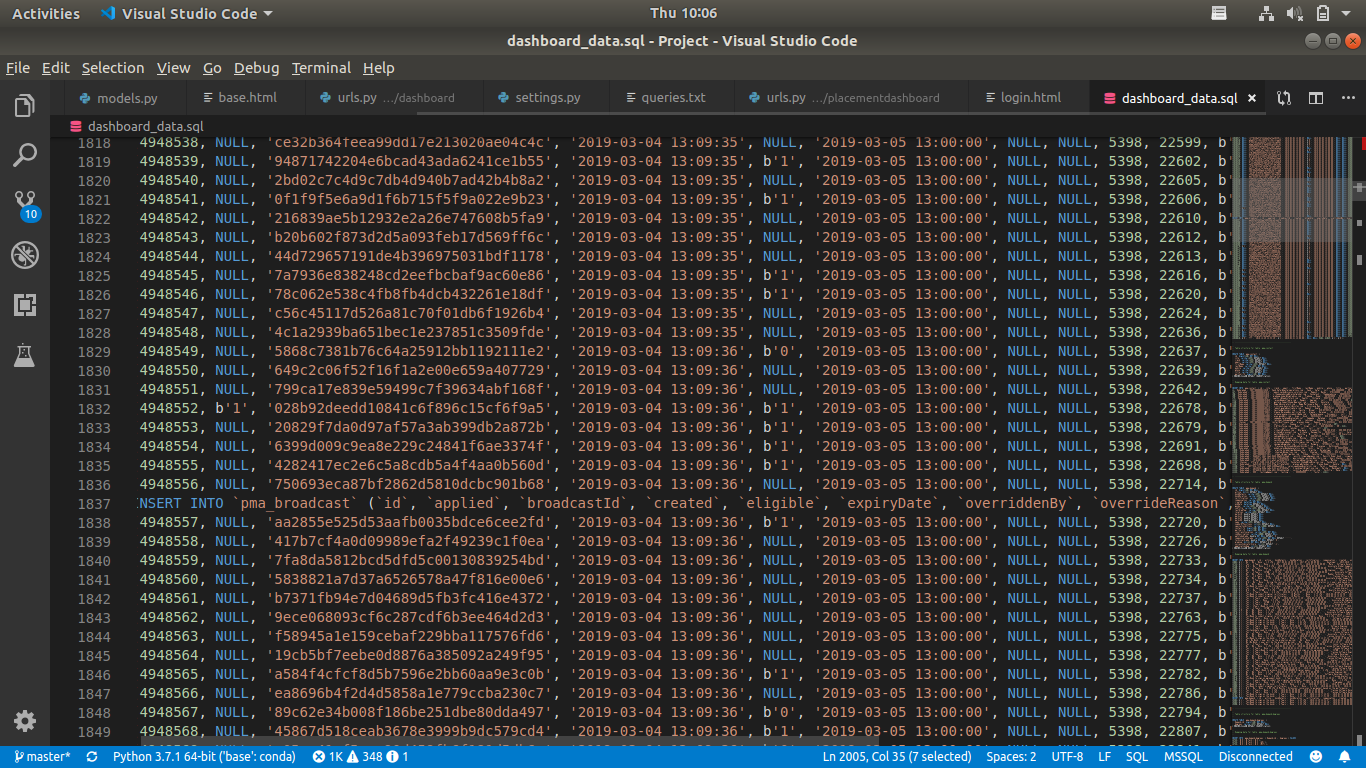
\includegraphics[width = 10cm]{images/8.png}
\end{center}
\end{frame}

\begin{frame}[plain]
\begin{center}
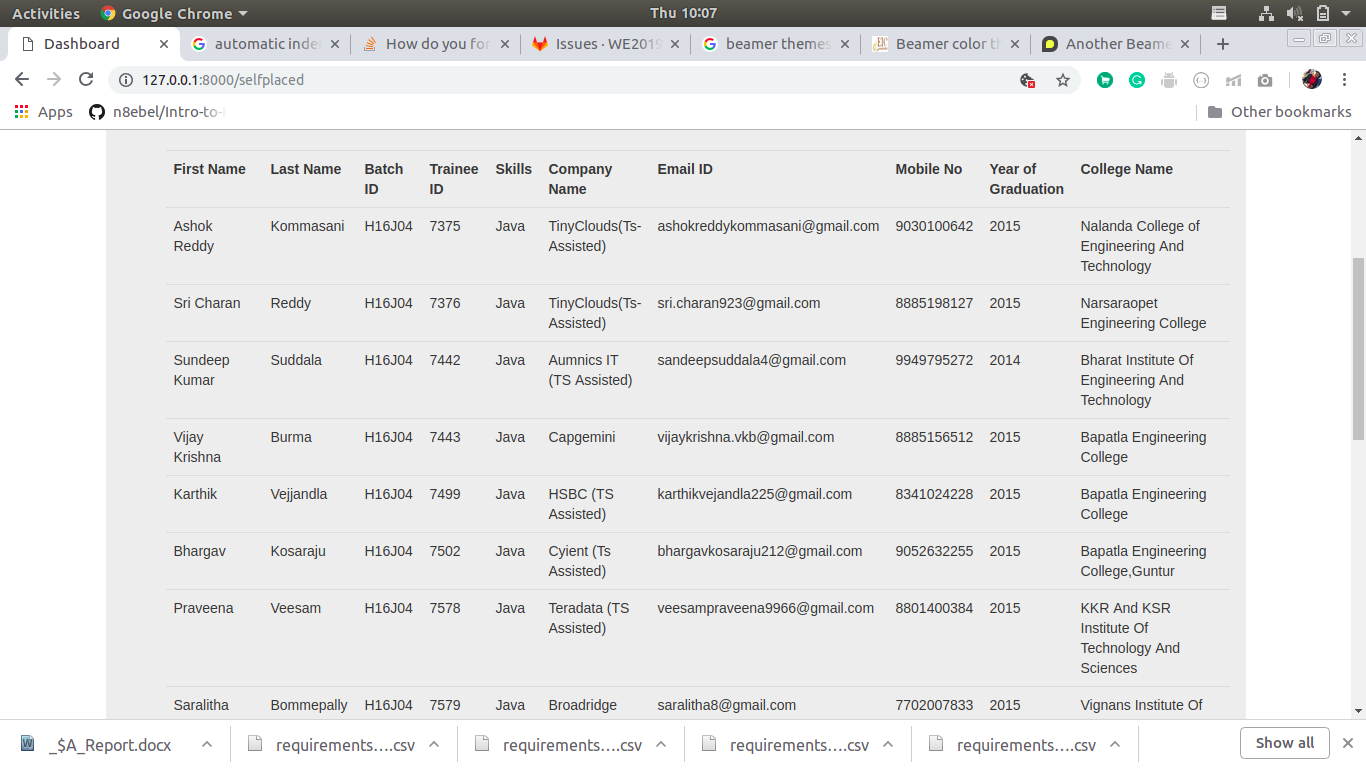
\includegraphics[width = 10cm]{images/9.png}
\end{center}
\end{frame}


\begin{frame}
\titlepage % Print the title page as the first slide
\end{frame}

%\begin{frame}
%\frametitle{ ~ Our objective} 
%\begin{itemize}
%\item{Enhancing knowledge of Python}
%\item{Exploring Python frameworks}
%\item{Delving into web technologies} 
%\end{itemize}
%\end{frame}

\begin{frame}
\frametitle{~ Description}
\begin {itemize}
\item{Placement data of TalentSprint}
\item{Pictorial representation of data}
\item{Easy analysis}
\end{itemize}
\end{frame}

\begin{frame}
\frametitle{ ~ Technology Stack} 
\begin {itemize}
\item Front-end
    \begin {itemize}
        \item{HTML} 
        \item{CSS}
        \item{JavaScript}
    \end{itemize}
\bigskip 
\item Back-end
    \begin {itemize}
        \item{Python} 
        \item{Python frameworks}
    \end{itemize}
\bigskip 
\item Database Management
    \begin {itemize}
        \item{MySQL}
    \end{itemize}
\end{itemize}
\end{frame}

\begin{frame}
\frametitle{ ~ Aim for the project week} 
\begin{itemize}
\item{Building dashboard using Django}
\item{Enhancing UI/UX}
\end{itemize}
\end{frame}



\begin{frame}
\frametitle{ ~ Current progress}
\begin{center}
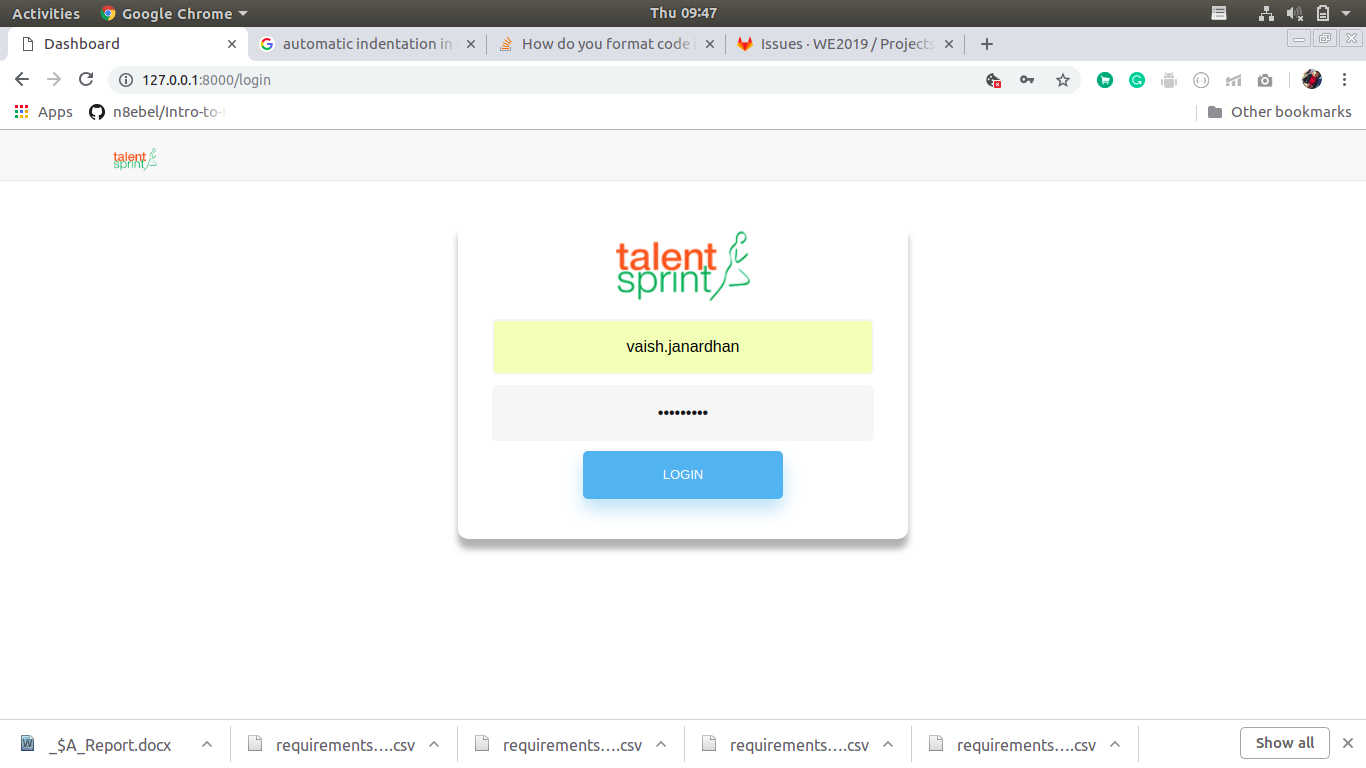
\includegraphics[width = 10cm]{images/1.png}
\end{center}
\end{frame}

\begin{frame}
\frametitle{ ~ Current progress}
\begin{center}
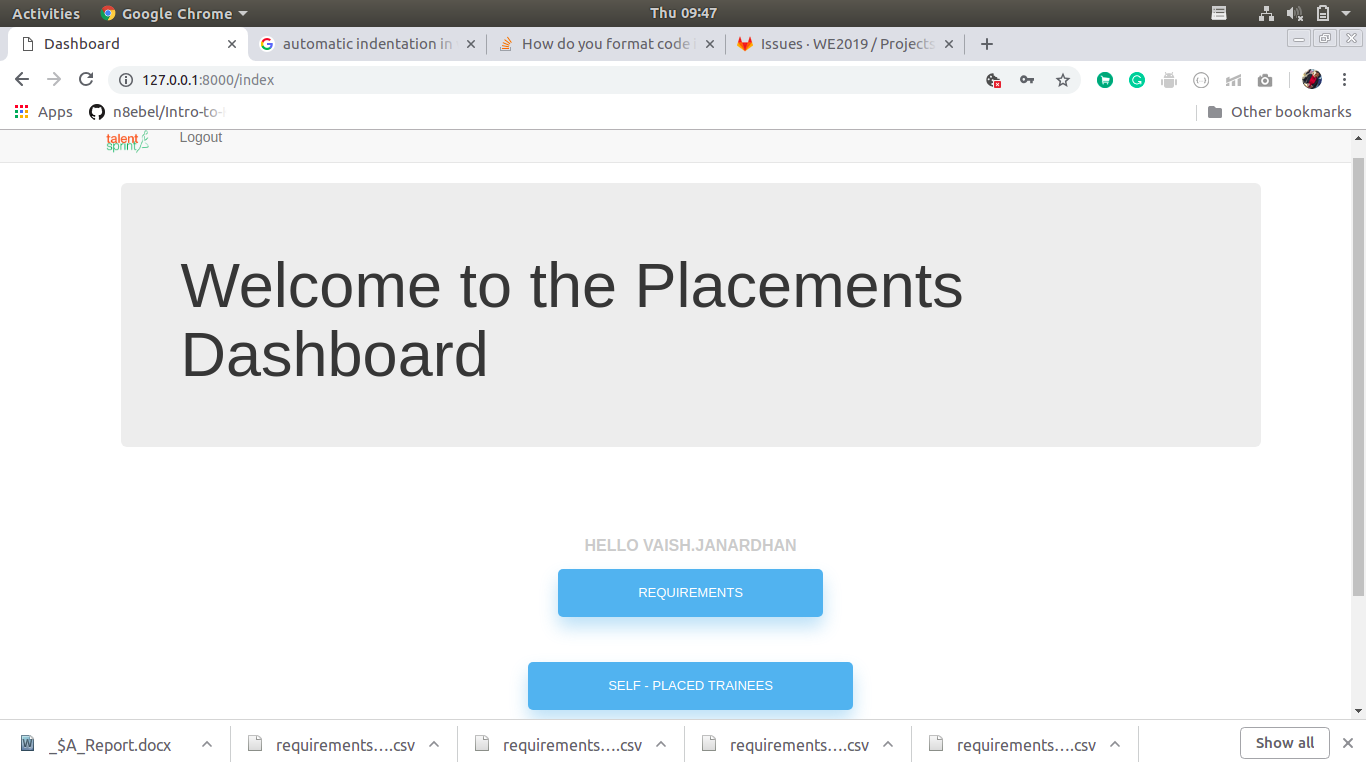
\includegraphics[width = 10cm]{images/2.png}
\end{center}
\end{frame}


\begin{frame}
\frametitle{ ~ Current progress}
\begin{center}
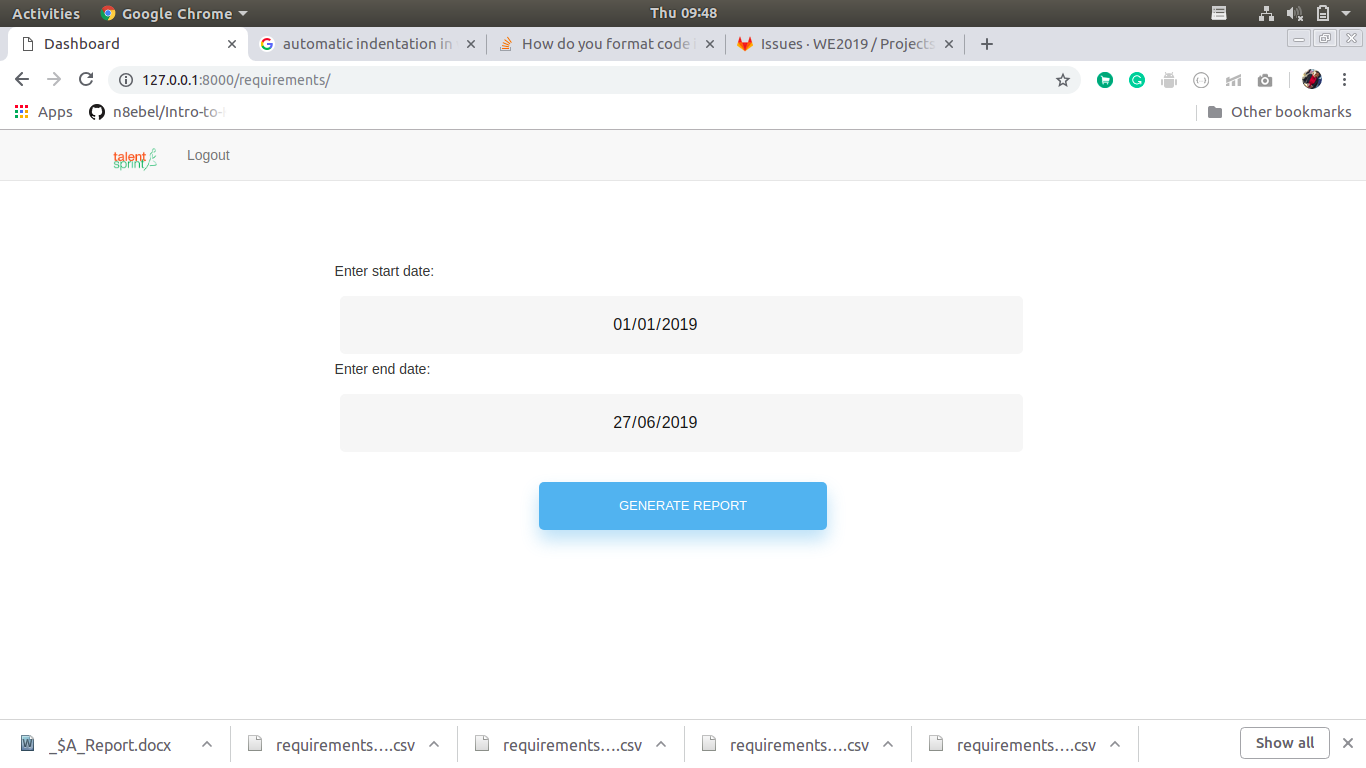
\includegraphics[width = 10cm]{images/3.png}
\end{center}
\end{frame}

\begin{frame}
\frametitle{ ~ Current progress}
\begin{center}
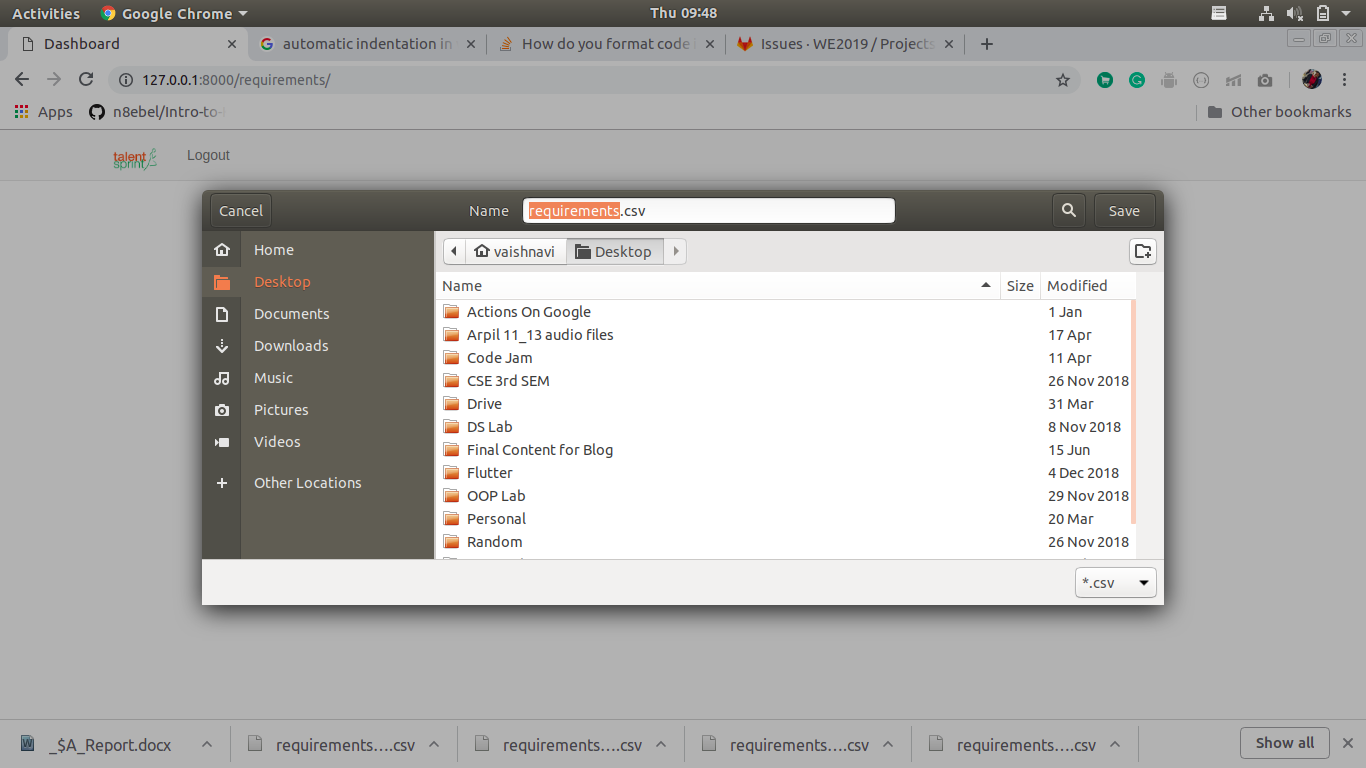
\includegraphics[width = 10cm]{images/4.png}
\end{center}
\end{frame}

\begin{frame}
\frametitle{ ~ Current progress}
\begin{center}
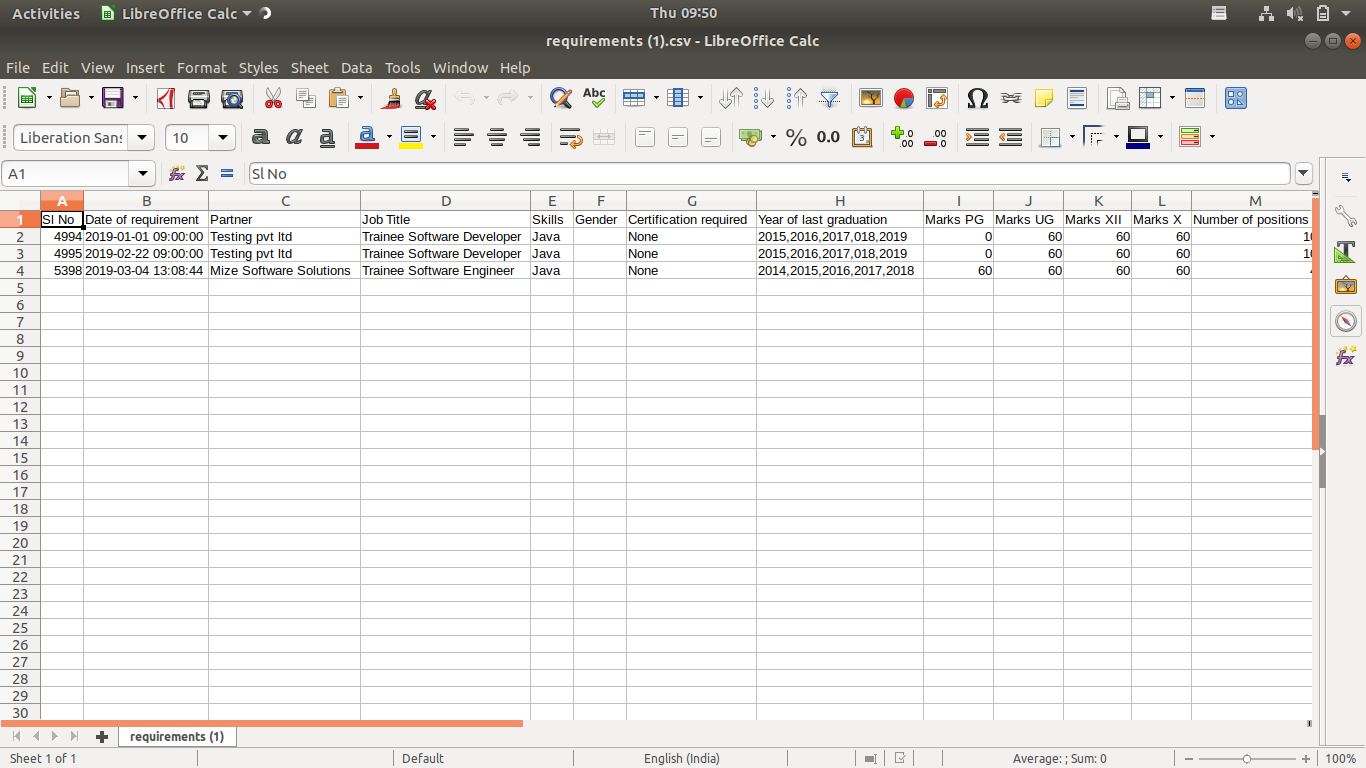
\includegraphics[width = 10cm]{images/5.png}
\end{center}
\end{frame}

\begin{frame}
\frametitle{ ~ Current progress}
\begin{center}
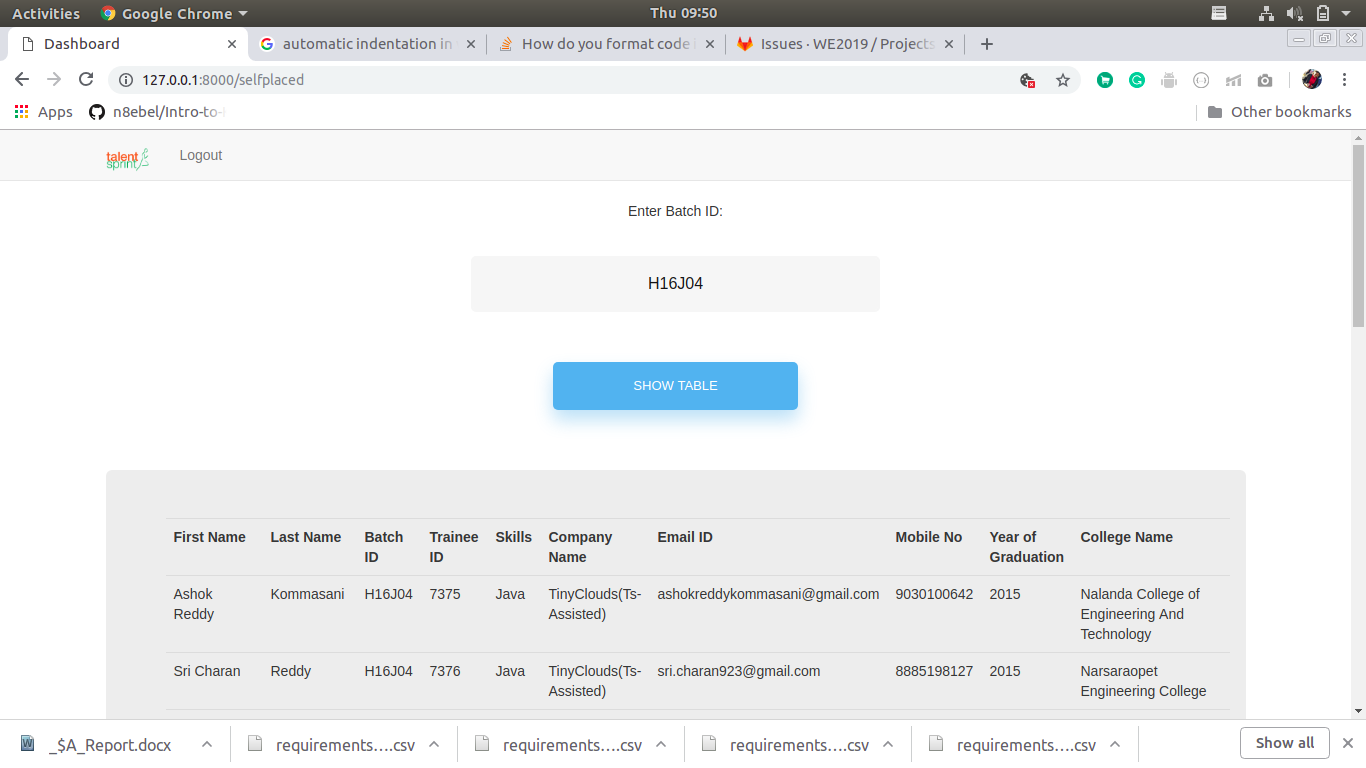
\includegraphics[width = 10cm]{images/6.png}
\end{center}
\end{frame}


\begin{frame}
\frametitle{ ~ Aim for today}
\begin{center}
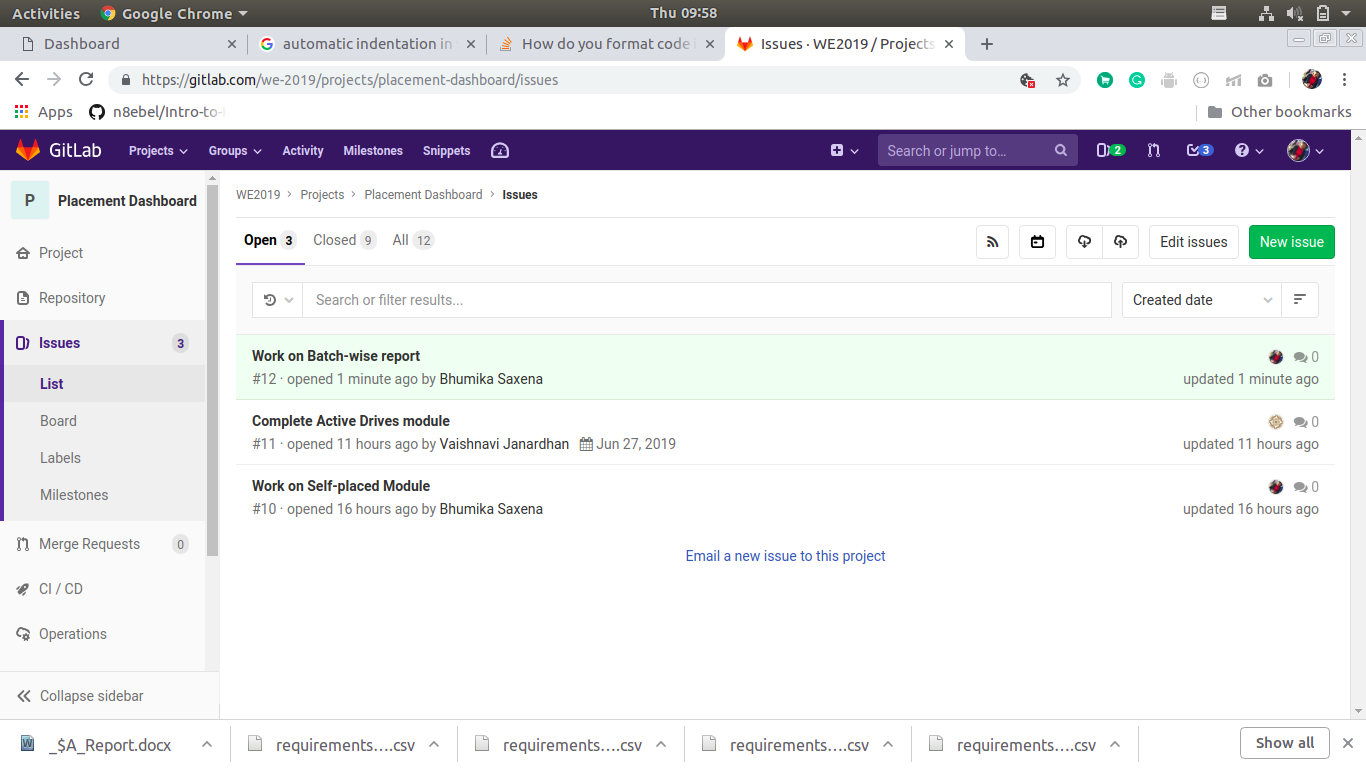
\includegraphics[width = 10cm]{images/7.png}
\end{center}
\end{frame}

\begin{frame}
\frametitle{ ~ Timeline}
\begin{center}
\begin{tabular}{|l|l|}
     \hline
     June 23 & Initial Setup\\
     \hline
     June 24 & Preparing the front-end skeleton\\
     \hline & Studying the database\\
     \hline
     June 25 & Connecting to database\\
     \hline & Showing response in tables\\
     \hline
     June 26 onwards & Extension to other modules\\
     \hline
     & Visualization using D3.js and Canvas\\
     \hline
     
\end{tabular}
\end{center}    
\end{frame}

\begin{frame}
\frametitle{ ~ Future Prospect} 
\begin{itemize}
\item{Using Pyramid}
\item{Comparing frameworks}
\item{Generating a detailed report}
\end{itemize}
\end{frame}


%------------------------------------------------

\begin{frame}
\begin{center}
\Huge{Discussion}
\end{center}
\end{frame}

%----------------------------------------------------------------------------------------

\end{document}